% Options for packages loaded elsewhere
\PassOptionsToPackage{unicode}{hyperref}
\PassOptionsToPackage{hyphens}{url}
%
\documentclass[
  11pt,
  ignorenonframetext,
]{beamer}
\usepackage{pgfpages}
\setbeamertemplate{caption}[numbered]
\setbeamertemplate{caption label separator}{: }
\setbeamercolor{caption name}{fg=normal text.fg}
\beamertemplatenavigationsymbolsempty
% Prevent slide breaks in the middle of a paragraph
\widowpenalties 1 10000
\raggedbottom
\setbeamertemplate{part page}{
  \centering
  \begin{beamercolorbox}[sep=16pt,center]{part title}
    \usebeamerfont{part title}\insertpart\par
  \end{beamercolorbox}
}
\setbeamertemplate{section page}{
  \centering
  \begin{beamercolorbox}[sep=12pt,center]{part title}
    \usebeamerfont{section title}\insertsection\par
  \end{beamercolorbox}
}
\setbeamertemplate{subsection page}{
  \centering
  \begin{beamercolorbox}[sep=8pt,center]{part title}
    \usebeamerfont{subsection title}\insertsubsection\par
  \end{beamercolorbox}
}
\AtBeginPart{
  \frame{\partpage}
}
\AtBeginSection{
  \ifbibliography
  \else
    \frame{\sectionpage}
  \fi
}
\AtBeginSubsection{
  \frame{\subsectionpage}
}
\usepackage{amsmath,amssymb}
\usepackage{lmodern}
\usepackage{iftex}
\ifPDFTeX
  \usepackage[T1]{fontenc}
  \usepackage[utf8]{inputenc}
  \usepackage{textcomp} % provide euro and other symbols
\else % if luatex or xetex
  \usepackage{unicode-math}
  \defaultfontfeatures{Scale=MatchLowercase}
  \defaultfontfeatures[\rmfamily]{Ligatures=TeX,Scale=1}
\fi
\usetheme[]{metropolis}
% Use upquote if available, for straight quotes in verbatim environments
\IfFileExists{upquote.sty}{\usepackage{upquote}}{}
\IfFileExists{microtype.sty}{% use microtype if available
  \usepackage[]{microtype}
  \UseMicrotypeSet[protrusion]{basicmath} % disable protrusion for tt fonts
}{}
\makeatletter
\@ifundefined{KOMAClassName}{% if non-KOMA class
  \IfFileExists{parskip.sty}{%
    \usepackage{parskip}
  }{% else
    \setlength{\parindent}{0pt}
    \setlength{\parskip}{6pt plus 2pt minus 1pt}}
}{% if KOMA class
  \KOMAoptions{parskip=half}}
\makeatother
\usepackage{xcolor}
\newif\ifbibliography
\usepackage{longtable,booktabs,array}
\usepackage{calc} % for calculating minipage widths
\usepackage{caption}
% Make caption package work with longtable
\makeatletter
\def\fnum@table{\tablename~\thetable}
\makeatother
\usepackage{graphicx}
\makeatletter
\def\maxwidth{\ifdim\Gin@nat@width>\linewidth\linewidth\else\Gin@nat@width\fi}
\def\maxheight{\ifdim\Gin@nat@height>\textheight\textheight\else\Gin@nat@height\fi}
\makeatother
% Scale images if necessary, so that they will not overflow the page
% margins by default, and it is still possible to overwrite the defaults
% using explicit options in \includegraphics[width, height, ...]{}
\setkeys{Gin}{width=\maxwidth,height=\maxheight,keepaspectratio}
% Set default figure placement to htbp
\makeatletter
\def\fps@figure{htbp}
\makeatother
\setlength{\emergencystretch}{3em} % prevent overfull lines
\providecommand{\tightlist}{%
  \setlength{\itemsep}{0pt}\setlength{\parskip}{0pt}}
\setcounter{secnumdepth}{-\maxdimen} % remove section numbering
\ifLuaTeX
  \usepackage{selnolig}  % disable illegal ligatures
\fi
\IfFileExists{bookmark.sty}{\usepackage{bookmark}}{\usepackage{hyperref}}
\IfFileExists{xurl.sty}{\usepackage{xurl}}{} % add URL line breaks if available
\urlstyle{same} % disable monospaced font for URLs
\hypersetup{
  pdftitle={Análisis de la asociación espacial},
  pdfauthor={Gerardo Martín},
  hidelinks,
  pdfcreator={LaTeX via pandoc}}

\title{Análisis de la asociación espacial}
\subtitle{Introducción}
\author{Gerardo Martín}
\date{2022-06-29}

\begin{document}
\frame{\titlepage}

\hypertarget{quuxe9-es-la-asociaciuxf3n}{%
\subsection{¿Qué es la asociación?}\label{quuxe9-es-la-asociaciuxf3n}}

\begin{frame}{¿Qué es la asociación?}
\begin{itemize}
\tightlist
\item
  Dos variables que se \emph{parecen}
\end{itemize}

\begin{longtable}[]{@{}rr@{}}
\toprule()
x & y \\
\midrule()
\endhead
1.1 & 3 \\
2.2 & 4 \\
3.3 & 5 \\
4.4 & 6 \\
5.5 & 7 \\
\bottomrule()
\end{longtable}
\end{frame}

\hypertarget{quuxe9-es-la-asociaciuxf3n-1}{%
\subsection{¿Qué es la asociación?}\label{quuxe9-es-la-asociaciuxf3n-1}}

\begin{frame}{¿Qué es la asociación?}
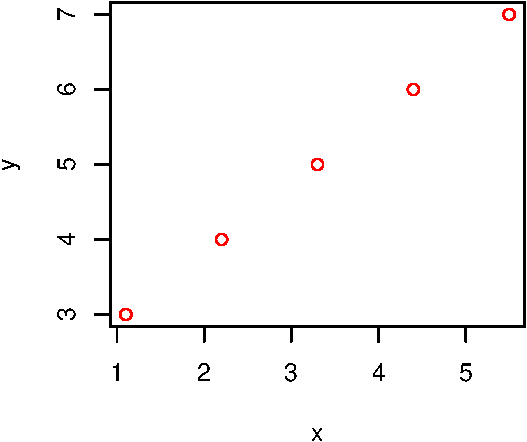
\includegraphics{Intro-asociacion_files/figure-beamer/unnamed-chunk-2-1.pdf}
\end{frame}

\hypertarget{quuxe9-es-la-asociaciuxf3n-2}{%
\subsection{¿Qué es la asociación?}\label{quuxe9-es-la-asociaciuxf3n-2}}

\begin{frame}{¿Qué es la asociación?}
\begin{itemize}
\item
  Variables se parecen, no porque sus valores sean iguales
\item
  Aumento de valores de una corresponden con aumento o disminución de la
  otra
\item
  Estadísticamente, indica que la varianza de una es explicada por otra
\item
  No implica causa-efecto
\end{itemize}
\end{frame}

\hypertarget{asociaciuxf3n-entre-variables-espaciales}{%
\subsection{Asociación entre variables
espaciales}\label{asociaciuxf3n-entre-variables-espaciales}}

\begin{frame}{Asociación entre variables espaciales}
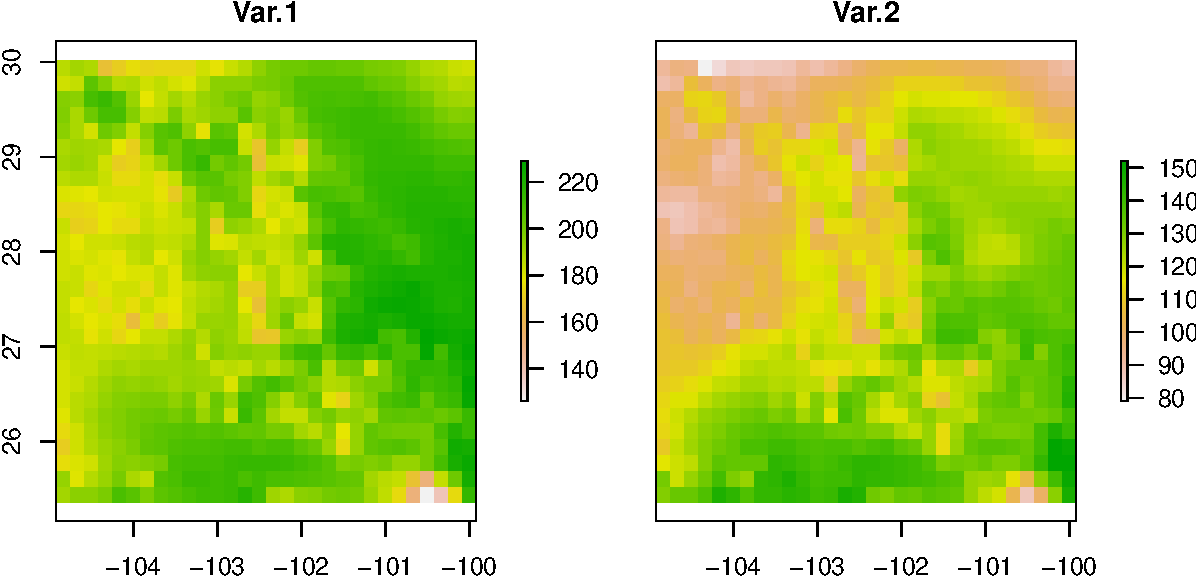
\includegraphics{Intro-asociacion_files/figure-beamer/unnamed-chunk-3-1.pdf}
\end{frame}

\hypertarget{asociaciuxf3n-entre-variables-espaciales-1}{%
\subsection{Asociación entre variables
espaciales}\label{asociaciuxf3n-entre-variables-espaciales-1}}

\begin{frame}{Asociación entre variables espaciales}
\begin{itemize}
\item
  Inspección visual puede ser insuficiente
\item
  Asociación, sólo en ciertas regiones
\item
  Es posible ver los valores en gráfico de dispersión
\end{itemize}
\end{frame}

\hypertarget{gruxe1fico-de-dispersiuxf3n-de-las-variables-raster}{%
\subsection{Gráfico de dispersión de las variables
raster}\label{gruxe1fico-de-dispersiuxf3n-de-las-variables-raster}}

\begin{frame}{Gráfico de dispersión de las variables raster}
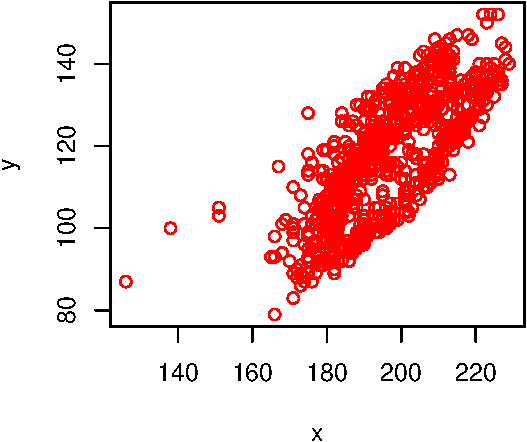
\includegraphics{Intro-asociacion_files/figure-beamer/unnamed-chunk-4-1.pdf}
\end{frame}

\hypertarget{asociaciuxf3n-entre-variables-espaciales-2}{%
\subsection{Asociación entre variables
espaciales}\label{asociaciuxf3n-entre-variables-espaciales-2}}

\begin{frame}{Asociación entre variables espaciales}
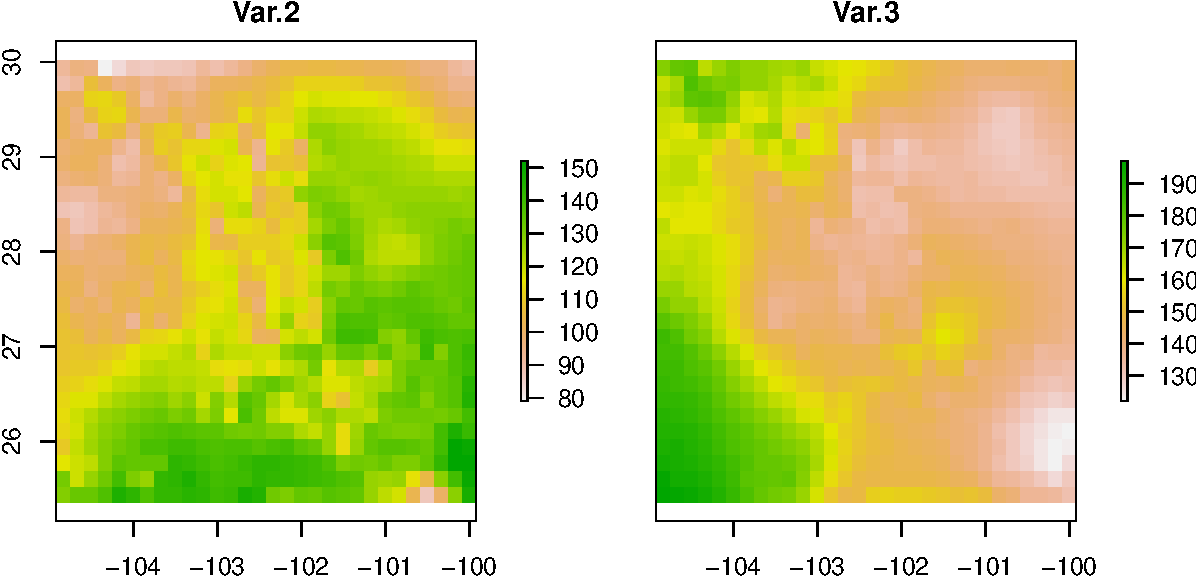
\includegraphics{Intro-asociacion_files/figure-beamer/unnamed-chunk-5-1.pdf}
\end{frame}

\hypertarget{gruxe1fico-de-dispersiuxf3n}{%
\subsection{Gráfico de dispersión}\label{gruxe1fico-de-dispersiuxf3n}}

\begin{frame}{Gráfico de dispersión}
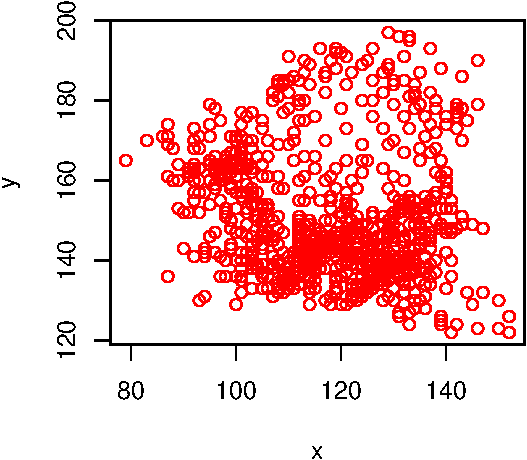
\includegraphics{Intro-asociacion_files/figure-beamer/unnamed-chunk-6-1.pdf}
\end{frame}

\hypertarget{anuxe1lisis-de-asociaciuxf3n-formal}{%
\subsection{Análisis de asociación
formal}\label{anuxe1lisis-de-asociaciuxf3n-formal}}

\begin{frame}{Análisis de asociación formal}
\begin{itemize}
\item
  Análisis gráfico, últil, insuficiente
\item
  No es objetivo
\item
  Necesario \emph{medir} la asociación
\item
  Pruebas estadísticas:

  \begin{itemize}
  \item
    Correlación
  \item
    Regresión
  \end{itemize}
\end{itemize}
\end{frame}

\end{document}
